% 请在下方的大括号相应位置填写正确的节标题和标签,以及作者姓名
\section{电荷密度与差分电荷密度}\label{sec:电荷密度与差分电荷密度}
\sectionAuthor{Jiaqi Z.}

% 请在下方的item内填写本节知识点
\begin{Abstract}
    \item 如何绘制电荷密度图
    \item 如何绘制差分电荷密度图
\end{Abstract}

% 请在正文相应位置填写正确的小节标题(或小小节标题),同时将标签的“节标题”和“小节标题”改为实际内容

这一节的内容并不难,但却是很多文献里都会放的一部分。在本节,我们将介绍如何绘制差分电荷密度图,很多文献都会通过这张图判断两个原子之间的成键性质,以及电荷转移情况。

\subsection{使用code{LCHARG}绘制电荷密度}\label{subsec:电荷密度与差分电荷密度-使用LCHARG绘制电荷密度}

本节我们要讨论的例子是NaCl这一典型材料,正如你在中学或大学了解到的那样,NaCl是离子晶体,其成键性质表现为Na失电子而Cl得电子。首先,我们需要构建出它的结构\footnote{Materials Project链接:https://next-gen.materialsproject.org/materials/mp-22862}:

\begin{lstlisting}[caption=POSCAR]
Na4 Cl4
1.0
    5.5881264354399347    0.0000000000000000    0.0000000000000003
    -0.0000000000000003    5.5881264354399347    0.0000000000000003
    0.0000000000000000    0.0000000000000000    5.5881264354399347
Na Cl
4 4
direct
    0.00  0.00  0.00 Na+
    0.00  0.50  0.50 Na+
    0.50  0.00  0.50 Na+
    0.50  0.50  0.00 Na+
    0.00  0.00  0.50 Cl-
    0.00  0.50  0.00 Cl-
    0.50  0.00  0.00 Cl-
    0.50  0.50  0.50 Cl-
\end{lstlisting}

首先进行考虑晶格常数的优化。完成后进行自洽计算,使用的\code{INCAR}如下所示:

\begin{lstlisting}[caption=INCAR]
ISTART =  1
ISPIN  =  1
LREAL  = .FALSE.
ENCUT  =  350
PREC   =  Accurate
LWAVE  = .FALSE.
LCHARG = .TRUE.
ADDGRID= .TRUE.
ISMEAR =  0
SIGMA  =  0.05
NELM   =  60
EDIFF  =  1E-5
\end{lstlisting}

与前面的自洽计算相比,要注意\keywordin{INCAR}{LCHARG}参数需要设置为\code{.TRUE.}表示\emph{输出\code{CHGCAR}文件}。计算完成后会得到\keyword{CHGCAR}文件。将其下载并在VESTA中打开,调整等值面大小(例如设置为0.05)并修改颜色,得到的电荷密度图如图\ref{fig:电荷密度与差分电荷密度-NaCl电荷密度}所示。可以发现,对NaCl而言,电子主要集中在Cl原子附近,这与我们前面对NaCl的认识一致。

\begin{figure}
    \centering
    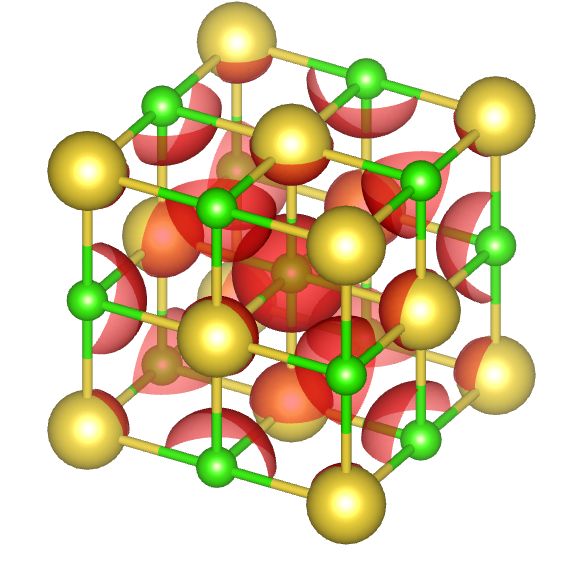
\includegraphics[width=0.7\linewidth]{VASP计算/静态自洽与电荷密度/电荷密度与差分电荷密度/fig/NaCl电荷密度.png}
    \caption{NaCl电荷密度}
    \label{fig:电荷密度与差分电荷密度-NaCl电荷密度}
\end{figure}

从数据的可视化角度出发,当然也可以使用二维数据,如图\ref{fig:电荷密度与差分电荷密度-二维NaCl电荷密度}所示,其结论与上面一致。只是从可视化角度可能更直观一点。

\begin{figure}
    \centering
    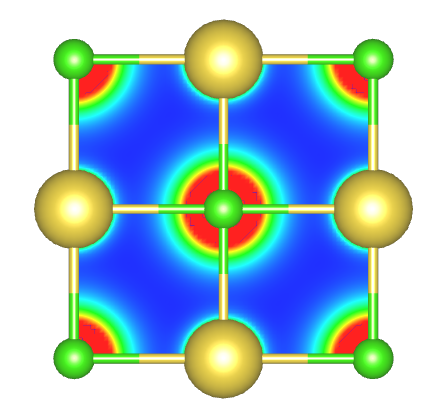
\includegraphics[width=0.7\linewidth]{VASP计算/静态自洽与电荷密度/电荷密度与差分电荷密度/fig/二维NaCl电荷密度.png}
    \caption{二维NaCl电荷密度}
    \label{fig:电荷密度与差分电荷密度-二维NaCl电荷密度}
\end{figure}

\subsection{绘制差分电荷密度图}\label{subsec:电荷密度与差分电荷密度-绘制差分电荷密度图}

下面我们要绘制差分电荷密度图,在绘制之前,我们首先需要明确;\emph{什么是差分电荷密度}。如果一个体系由两部分A和B组成,其总电荷分布为$\rho$,当仅存在A体系时的电荷分布为$\rho_A$,类似地仅存在B体系时地电荷分布为$\rho_B$。则差分电荷密度定义为

\begin{equation*}
    \Delta\rho = \rho - \rho_A - \rho_B
\end{equation*}

可以发现,\emph{当某个地方的电荷数增多时,差分电荷为正,反之,当电荷减少时,差分电荷为负}。也可以发现,在计算差分电荷密度之前,我们首先需要有三个体系的电荷密度(AB体系、A体系、B体系)。每一个体系的差分电荷计算都如上面所介绍的方法一样。采用类似的方法,得到三个体系的电荷密度。

\begin{attention}
    在计算不同体系的电荷密度时,不需要进行结构优化,而直接在AB体系中删去另一个体系的原子即可。

    此外,在计算时应当保持参数一样,尤其是k点密度。
\end{attention}

在本例中,A、B体系分别是Na原子和Cl原子组成的体系,计算得到电荷密度后可以直接使用\code{vaspkit-314}“Charge-Density Difference”功能,分别输入AB体系、A体系和B体系的\code{CHGCAR}文件(使用相对路径\footnote{也许你已经忘记相对路径是什么了,可以回到Linux部分的\ref{subsec:认识Linux目录-绝对路径和相对路径}一节。}),会得到\code{CHGDIFF.vasp}文件,将其用VESTA打开,调整可视化选项,即可得到差分电荷密度图如图\ref{fig:电荷密度与差分电荷密度-NaCl差分电荷密度}所示。可以发现,在Cl原子附近电荷增多,表现为得电子。

\begin{figure}
    \centering
    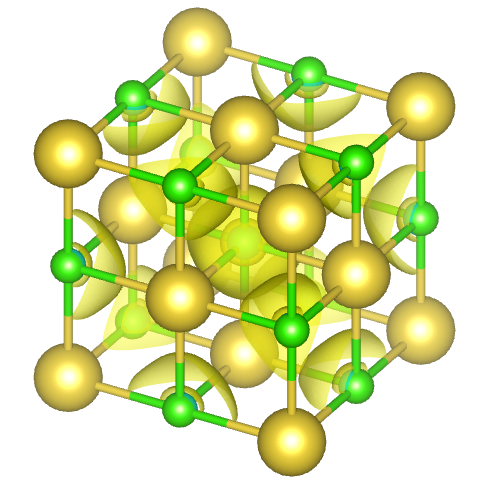
\includegraphics[width=0.7\linewidth]{VASP计算/静态自洽与电荷密度/电荷密度与差分电荷密度/fig/NaCl差分电荷密度.png}
    \caption{NaCl差分电荷密度}
    \label{fig:电荷密度与差分电荷密度-NaCl差分电荷密度}
\end{figure}

与电荷密度类似,这里也可以绘制二维甚至一维差分电荷密度图(也可以叫\emph{平面平均差分电荷密度图})。

\subsubsection{*如何绘制平面平均差分电荷密度图}

\emph{平面平均差分电荷密度图},指的是对某一平面内的差分电荷密度做平均计算,并绘制沿另一个方向(通常是$z$轴)的变化曲线。例如,在二维材料里(比如异质结),通过这种方法可以看出不同材料之间在界面处的电荷转移情况(如图\ref{fig:电荷密度与差分电荷密度-平面平均差分电荷密度图}所示\footnote{参考文献:Xia, C. et al. J. Mater. Chem. A 5, 13400–13410 (2017). https://doi.org/10.1039/C7TA02109G})。

\begin{figure}
    \centering
    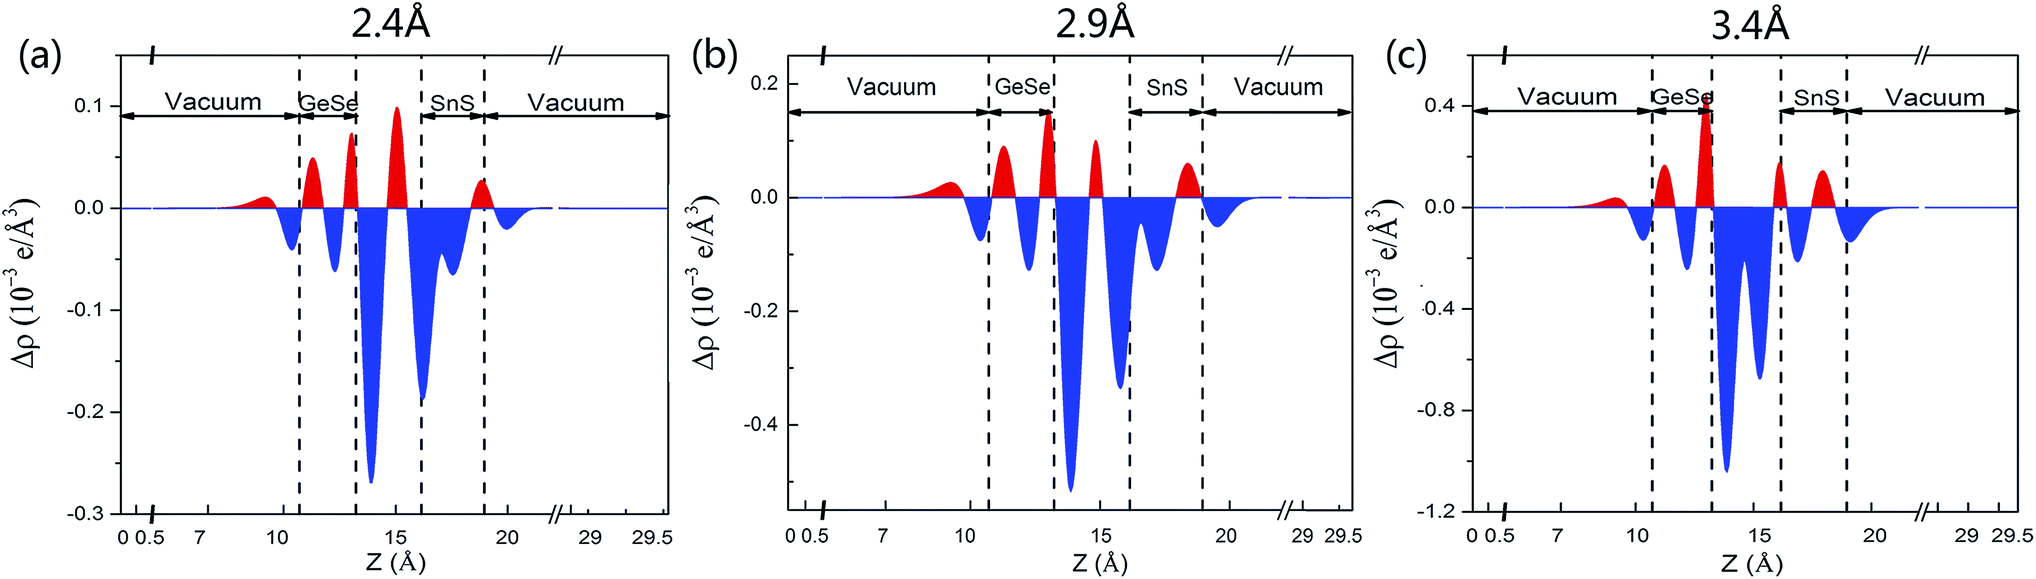
\includegraphics[width=1\linewidth]{VASP计算/静态自洽与电荷密度/电荷密度与差分电荷密度/fig/平面平均差分电荷密度图.png}
    \caption{平面平均差分电荷密度图}
    \label{fig:电荷密度与差分电荷密度-平面平均差分电荷密度图}
\end{figure}

\begin{attention}
    一般来说,平面平均差分电荷密度图用于二维材料相互作用,且绘制方向通常沿着真空层方向。在本例中,我们尽管可以绘制某种平面平均差分电荷密度图,但没有什么明显结论,仅作为步骤演示,不展示结果。
\end{attention}

在绘制的时候,首先需要在当前计算差分电荷密度的目录(即有\code{CHGDIFF.vasp}文件的目录),使用\code{vaspkit-316}“1D Planar-Average Charge Density”功能,选择\code{3-Specified Charge Density File}并输入\code{CHGDIFF.vasp}(差分电荷密度文件),完成后会生成\code{PLANER\_AVERAGE.dat}文件,将其放入origin作图即可。





% \subsection{错误处理}\label{subsec:节标题-错误处理}
% % 请在本节列出可能遇见的错误与解决方法

% \subsubsection{错误1}

% \subsubsection{错误2}

% \subsubsection{错误3}